\section{Vision Transformer vs. CNN}

\begin{frame}{ViT vs. CNN}
    \begin{itemize}
        \item Local vs. Global Understanding: While CNNs are good at local feature extraction, ViT captures global relationships from the very first layer.
	    \item Efficiency on Large Datasets: ViT shines on large datasets, while CNNs, due to their inductive biases (local patterns, translation invariance), perform better on smaller datasets without needing as much data.
	    \item Simplicity in Architecture: ViT uses a simpler architecture with fewer specialized layers, while CNNs rely on task-specific layers like convolutions and pooling.
    \end{itemize}
\end{frame}

\begin{frame}{Combining CNNs and Transformers}
    \begin{itemize}
        \item As an alternative to raw image patches, the input sequence can be formed from feature maps of a CNN.
	    \item These hybrid models combine the local feature extraction capabilities of CNNs with the global context awareness of Transformers. 
        \item These models can perform well even on smaller datasets.
    \end{itemize}
\end{frame}

\begin{frame}{Dataset Size}
    \begin{columns}
        \begin{column}{0.5\textwidth}
            \begin{figure}
                \centering
                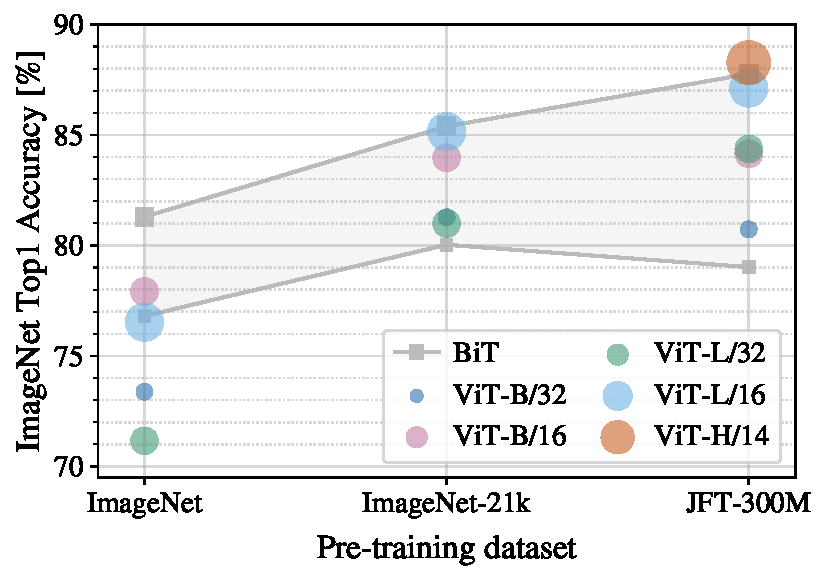
\includegraphics[width=\textwidth]{pic/transvolution-i1k-scaling}
                \caption{
                % Transfer to ImageNet. 
                While large ViT models perform worse than BiT ResNets when pre-trained on small datasets, they shine when pre-trained on larger datasets. 
                %Similarly, larger ViT variants overtake smaller ones as the dataset grows.
                }
                \label{fig:transvolution}
            \end{figure}
        \end{column}
        \begin{column}{0.5\textwidth}
            \begin{figure}
                \centering
                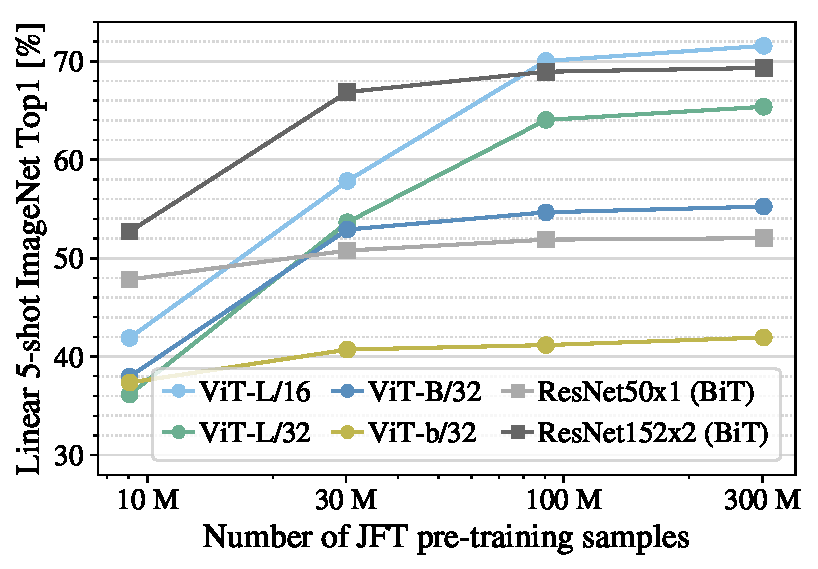
\includegraphics[width=\textwidth]{pic/imagenet_5shot}
                \caption{
                % Linear few-shot evaluation on ImageNet versus pre-training size. 
                ResNets perform better with smaller pre-training datasets but plateau sooner than ViT, which performs better with larger pre-training. 
                %ViT-b is ViT-B with all hidden dimensions halved.
                }
                \label{fig:imagenet_5shot}
            \end{figure}
        \end{column}
    \end{columns}
\end{frame}


\begin{frame}{Performance versus Pre-training}
    \begin{figure}
        \centering
        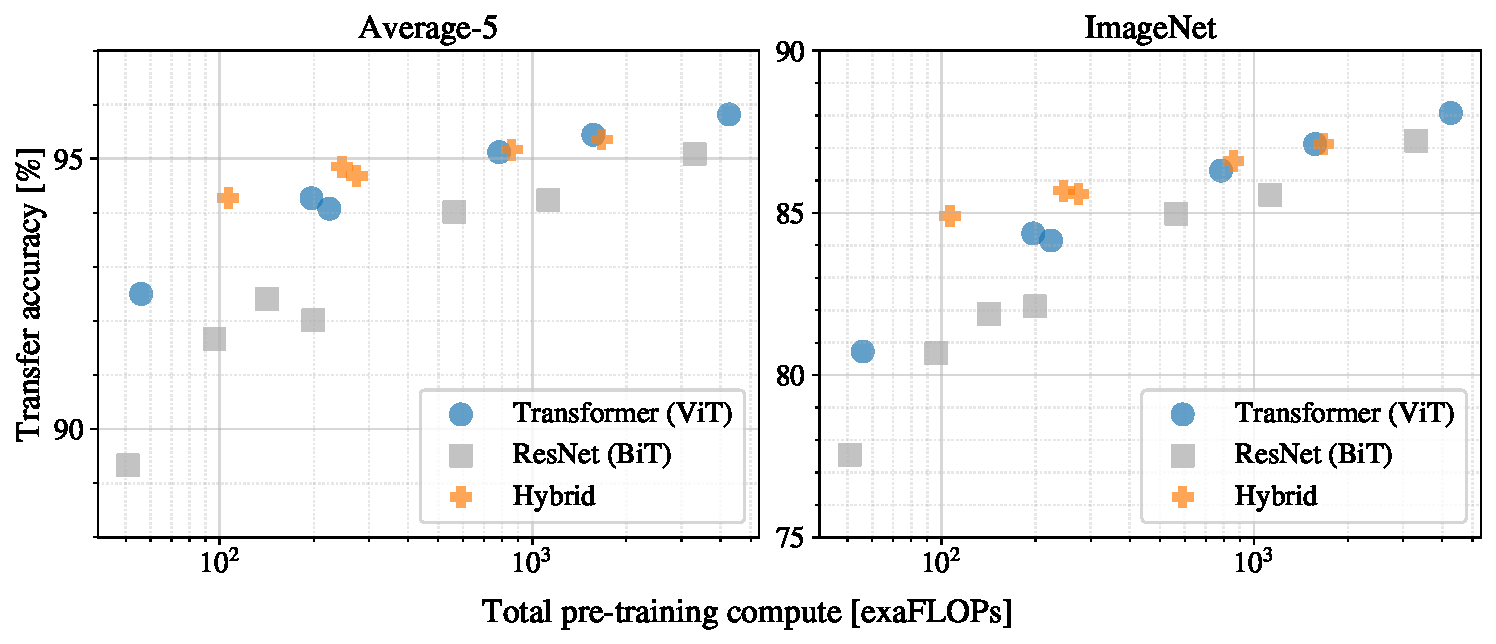
\includegraphics[width=0.9\linewidth]{pic/finetune_vs_compute2.pdf}
        \caption{Vision Transformers generally outperform ResNets with the same computational budget. Hybrids improve upon pure Transformers for smaller model sizes, but the gap vanishes for larger models.}
        \label{fig:enter-label}
    \end{figure}
\end{frame}